Trajectory prediction and planning for autonomous vehicles must produce behavior that is not only geometrically accurate but also safe, legal, and socially compliant. Modern deep multi-modal predictors—including anchor-based methods, latent-variable generators, and diffusion-based samplers—can generate diverse candidate futures. However, the selection of the final executed trajectory remains an underspecified stage in most systems. When several plausible modes exist, the system must choose one that satisfies explicit, priority-ordered traffic rules.

This paper addresses that problem by introducing \textsc{RECTOR} (\textbf{R}ule-\textbf{E}nforced \textbf{C}onstrained \textbf{T}rajectory \textbf{OR}chestrator), a rule-aware selection framework that ranks candidate ego trajectories using a tiered rulebook and a tolerance-based lexicographic ordering.  The framework is built around three components: (i)~a neural head that predicts \emph{which rules apply} in a given scene, (ii)~differentiable smooth proxies that evaluate \emph{how severely} each applicable rule is violated, and (iii)~a deterministic lexicographic selector that enforces the non-negotiable priority hierarchy Safety~$\succ$~Legal~$\succ$~Road~$\succ$~Comfort.  Because RECTOR operates entirely at selection time, it is architecturally compatible with upstream multi-modal trajectory generators without modifying the predictor itself, and its empirical value should be interpreted as reranking the same candidate set rather than repairing the generator.

The primary empirical result is that, even though confidence-only selection already yields no reported Protocol~A violation in 76.14\% of scenarios, rule-aware selection---whether lexicographic or weighted-sum---still changes which candidate is executed in the minority of hard scenes: selected-mode compliance rises to 84.97\%, total violations fall by 8.83~pp, and the gain is concentrated in Safety-tier tail-risk filtering rather than broad correction of benchmark-wide behavior.  On the current benchmark, the lexicographic selector produces identical binary compliance outcomes to weighted-sum across all 250 tested weight configurations (including fully flat weights $w_S{=}w_C{=}1$, which diverge by exactly 1~scenario out of 12{,}800); adversarial confidence injection likewise confirms that both rule-aware strategies reject safety-violating candidates at the same rate (3.6--5.7\%) while confidence-only selection fails at 100\%.  These experiments establish that the empirical lex--WS equivalence is a structural property of the WOMD validation distribution (Safety proxy scores are large, median~$\approx 1.0$; cross-tier Comfort advantages are small, effective misspecification boundary at $w_S/w_C\approx1$) rather than an artifact of the tested weight range.  RECTOR's lexicographic formulation contributes (i) a formal guarantee that higher-priority violations cannot be traded for lower-priority gains independent of score scale, weight specification, or distribution of compliance margins---a guarantee that weighted-sum satisfies only when weights are correctly calibrated---and (ii) complete elimination of weight tuning from the selector, which matters when calibration data are scarce, the score distribution shifts, or auditability of the decision is required.  The following subsections elaborate on this motivation, outline the concrete contributions, and define the scope of the current work.

%-------------------------------------------------------------------------------
\subsection{Motivation: The Compliance Gap}
\label{subsec:motivation}
%-------------------------------------------------------------------------------

To illustrate the selection problem, consider standard metrics such as Minimum Average Displacement Error (minADE).  While these metrics measure how well predictions cover the ground truth, they do not assess the safety or legality of the executed mode.  In complex scenes, two candidates may be geometrically similar yet critically different: one might violate a red light or fail to yield even with a low geometric error.  This discrepancy is especially pronounced in ``long-tail'' interactive scenarios, where error distributions are heavy-tailed (Fig.~\ref{fig:percentile_analysis}).  In these regimes, selection is not a minor post-processing step but a primary mechanism for ensuring plan acceptability.

%-------------------------------------------------------------------------------
\subsection{Key Technical Observations}
\label{subsec:observations}
%-------------------------------------------------------------------------------

RECTOR’s design is motivated by four technical observations. First, traffic rules follow a strict priority structure: safety dominates legality, which in turn dominates road-level and comfort considerations.  Unlike scalar penalties, lexicographic ordering ensures that higher-priority tiers are never traded off for lower-priority gains. Second, rule applicability is context-dependent: a stop-sign rule is irrelevant without a stop sign.  Rather than relying on brittle hand-coded logic, \textsc{RECTOR} uses a learned model to predict the ``active rule set'' directly from scene features. Third, many rules admit smooth approximations; core constraints such as collision margins can be expressed as continuous proxy functions for numerically stable scoring.

Fourth, \emph{when no candidate satisfies high-priority constraints, the system must degrade gracefully}. A finite candidate set may not always contain a fully compliant option.  In such cases, the selector should choose the \emph{least-violating} trajectory and signal infeasibility to downstream components, rather than falling back to confidence-only selection.  We formalize this as a minimum-violation fallback with an explicit infeasibility flag (Section~\ref{subsec:formal_guarantees}).

%-------------------------------------------------------------------------------
\subsection{Approach Overview}
\label{subsec:approach}
%-------------------------------------------------------------------------------

Taken together, these observations suggest a two-stage architecture. In the reference instantiation used in this paper, a Transformer--CVAE generator inspired by the M2I interactive prediction family generates $K=6$ candidate ego trajectories over a fixed 5-second horizon ($T=50$ timesteps at 10\,Hz). Each mode is a sequence of ego states with a confidence score~\cite{Sun_2022}.  RECTOR's rule-aware selection layer is decoupled from the generator and can be attached to the candidate set produced upstream.

In the second stage, each candidate is evaluated against a catalog of $R{=}28$ traffic rules organized into four tiers that reflect the normative priority structure motivated in Section~\ref{subsec:observations}.  The four tiers are:
\begin{itemize}[leftmargin=1.5em] 

\item \textbf{Safety (Tier~0):} collision avoidance and minimum distance
constraints (5~rules), 

\item \textbf{Legal (Tier~1):} traffic-signal and stop-sign compliance, speed limits, and right-of-way rules (7~rules),\footnote{Tier labels are used as research abstractions within the WOMD-based rule catalog; deployment and jurisdictional qualifications are discussed in Sections~\ref{Sec:Known_Gaps_and_Next_Steps_Toward_Deployment} and~\ref{Sec:Conclusion}.}


\item \textbf{Road (Tier~2):} lane keeping and road boundary adherence
(2~rules), \item \textbf{Comfort (Tier~3):} acceleration, jerk, and steering bounds
and smooth motion preferences (14~rules).

\end{itemize}

\noindent
Candidates are then ranked by tolerance-based lexicographic ordering. The selector minimizes Safety-tier violations first. Only near-ties, within a small tolerance, are resolved using the Legal tier, then the Road tier, and finally the Comfort tier. This procedure makes priorities explicit and removes weight tuning from the selector itself. In particular, a small improvement in comfort can never displace a safer or more lawful candidate. The result is a deterministic, auditable decision based only on tier scores and tolerance parameters, not on tuned scalar weights.

%-------------------------------------------------------------------------------
\subsection{Contributions}
\label{subsec:contributions}
%-------------------------------------------------------------------------------

Against this background, the specific contributions of this paper are as follows.

\begin{enumerate}[label=\textbf{C\arabic*},leftmargin=2.5em]

\item \textbf{Negative Result on Applicability Learning with Immediate Deployment Implications.} We systematically compare four applicability policies---learned head, hybrid conservative (always-on for Safety/Legal, learned for Road/Comfort), fully always-on, and oracle---under cross-evaluation on 43{,}219 scenarios (Table~\ref{tab:conservative_applicability}).  The central finding is negative but practically important: a \emph{parameter-free always-on policy strictly dominates} the 3.33\,M-parameter learned head on \emph{both} Safety-tier compliance ($-$2.64~pp: 23.06\%\,$\to$\,20.43\%) \emph{and} selected-trajectory accuracy ($-$0.089\,m selADE: 2.138\,$\to$\,2.049\,m).  The accuracy improvement occurs because activating more Safety rules steers the selector away from collision-prone, geometrically extreme modes.  We therefore recommend always-on activation for Safety and Legal tiers as the default deployment policy and treat the learned head as residual support for Road and Comfort tiers, where false-positive activation incurs measurable accuracy cost.  The learned head's failure on Safety-tier rules is a class-imbalance problem: per-rule F1 is almost entirely determined by oracle support ($\rho{=}0.994$); rules with $>$5{,}000 positive instances achieve mean $\text{F}_1{=}0.75$ while rules below 1{,}000 achieve $\text{F}_1{=}0.00$.  This finding has direct practical implications: for safety-critical tiers, a parameter-free conservative policy should be preferred over learned prediction until recall on rare Safety events is substantially improved.

\item \textbf{Practical Rule-Aware Selection Integration Beyond Prior Rulebooks.} Building on the lexicographic rulebook concept of Censi~et~al., we integrate priority-ordered selection into a learned multi-modal trajectory pipeline.  The concrete additions beyond prior rulebook formulations are the learned applicability head, differentiable proxies for 24 of 28 rules, and a batched selector compatible with GPU inference while preserving the intended hierarchy.  The measured benefit is a reranking effect on the same candidate set, with most of the headroom coming from avoiding Safety-tier tail-risk selections rather than from broad changes in an already mostly compliant benchmark.

The primary empirical result is that \emph{rule-aware selection of any kind} raises selected-mode compliance from 76.14\% to 84.97\% and reduces Safety+Legal violations from 21.87\% to 13.15\% on 12{,}800 scenarios.  On this benchmark, weighted-sum and RECTOR produce near-identical binary compliance outcomes: extending the weight grid to 250 configurations (including fully flat weights $w_S{=}w_C{=}1$) shows that WS diverges from lex on at most 1 scenario out of 12{,}800 ($+$0.0078~pp) and matches lex exactly for $w_S \geq 5$; the 0.100\,m selADE gap in favour of weighted-sum is a tie-breaking artefact explained in Section~\ref{subsubsec:selected_accuracy}.  Adversarial confidence injection (Section~\ref{subsubsec:adversarial}) confirms that both rule-aware strategies reject safety-violating candidates at the same rate (3.6--5.7\%) while confidence-only selection picks the injected violator at 100\%: the separation is rule-aware vs.\ confidence-only, not lexicographic vs.\ weighted-sum.  Because the benchmark already contains many compliant or near-compliant modes, the relevant gain is the ability to filter the unsafe tail of the candidate set, not to convert a broadly unlawful predictor into a lawful one.

The contribution of lexicographic ordering is therefore not a measurable compliance gain on this distribution, but a \emph{structural guarantee that holds independent of score scale and weight values}: lexicographic selection provably cannot trade a higher-priority violation for a lower-priority gain regardless of how the proxy scores are scaled or distributed.  Weighted-sum satisfies this property only when weights are correctly calibrated (here, $w_S \geq 5 w_C$); below that threshold it can fail.  Lexicographic selection requires no weight specification and cannot be miscalibrated, which matters in deployment contexts where calibration data are scarce, scores shift under distribution shift, or the decision must be fully auditable without reference to tuned parameters.

\item \textbf{Correctness Properties of the Selector.} We verify three properties of \textsc{RECTOR}'s deterministic selector: order invariance (selection is independent of candidate input order), infeasibility fallback (minimum-violation selection when no fully compliant candidate exists), and scalarization correctness (a sufficiently large exponential base recovers lexicographic ranking from a scalar score; this condition is automatically satisfied by the tier-score normalization contract for any base $B > 3$).  These are straightforward consequences of the selector's definition and of known results in lexicographic optimization~\cite{Ehrgott2005}, but we state and verify them explicitly to support reproducibility.  The infeasibility fallback is proven formally and the implementation now emits an explicit \texttt{infeasible} flag when the selected candidate has non-zero Safety-tier score, enabling downstream fail-safe logic.  Empirically, tolerance sweeps from $10^{-3}$ to $10^{-2}$ leave Safety, Legal, and total violations unchanged, confirming robustness to implementation parameters.

\item \textbf{Differentiable Proxy Catalog for Selection-Time Enforcement.} We implement 24 differentiable proxy functions spanning Safety, Legal, Road, and Comfort constraints, enabling continuous rule severity scoring for batched selection-time enforcement while keeping 4 semantically difficult rules reserved for post-hoc audit.  Proxy--full-evaluator alignment shows mean pairwise candidate-ranking concordance of 0.948 across all 24~proxied rules (0.875 for the 10~rules with measurable variance in both evaluators; 1{,}000 scenarios), indicating that the proxy reliably preserves tier-aggregate candidate ordering despite moderate per-rule severity correlations (mean Spearman $\rho{=}0.25$) (Section~\ref{Sec:Rule_Evaluation_And_Data_Pipeline}).

\item \textbf{Verification Pipeline for Rule-Aware Selection.} We complement the proxy layer with a verification pipeline covering semantic invariants (non-negativity, correct applicability gating, monotonicity, temporal consistency), numerical stability (0.0\% post-mitigation NaN/Inf rate), and proxy--auditor alignment.  A 55-scenario Waymax log-replay validation over 3{,}338.5\,s reports zero overlap steps and confirms end-to-end simulator-bridge execution.  Robustness experiments show that injected perception and map perturbations increase violation rates in a controlled, bounded manner (up to ${\sim}$6.1\,pp for perception noise, ${\sim}$12.1\,pp for worst-case map errors), demonstrating that the pipeline's checks meaningfully bound failure modes (Section~\ref{Sec:Section_VIII_Verification_Invariants_Numerical_Stability_and_Integration_Tests}).

\item \textbf{Empirical Validation.} On 12{,}800 WOMD \texttt{validation\_interactive} scenarios, \textsc{RECTOR} shows that nontrivial selection headroom remains even when the candidate set is already mostly compliant: reported selected-mode compliance rises from 76.14\% to 84.97\% (23.86\%\,$\to$\,15.03\% total violations, about 1.1k fewer violating executed trajectories).  The Safety tier provides the dominant improvement (21.87\%~$\to$~13.15\%, $-$8.72~pp) under the learned applicability head, which is the strongest evidence that the remaining headroom lies in tail-risk filtering rather than in correcting pervasive rule breaking; a uniformly weighted-sum baseline achieves numerically identical outcomes on this evaluation set.  Scope boundaries, deployment qualifications, and failure modes are consolidated in Sections~\ref{Sec:Known_Gaps_and_Next_Steps_Toward_Deployment} and~\ref{Sec:Conclusion}.

\end{enumerate}

%-------------------------------------------------------------------------------
\subsection{System Architecture}
\label{subsec:architecture}
%-------------------------------------------------------------------------------

RECTOR augments standard multi-modal generators with two rule-aware modules (Fig.~\ref{fig:rector_architecture}).  First, an \textbf{applicability mechanism} identifies active constraints from the scene embedding—for example, triggering stop-sign rules only at intersections and crosswalk-yield rules when pedestrians are present.  In the reference model this mechanism is learned, but the results later show that always-on activation is the preferable default for Safety and Legal tiers on the current benchmark.  Second, a \textbf{tiered lexicographic scorer} aggregates these violations and selects the candidate with the minimal tier-score vector.  This architecture is intentionally modular: while the generator focuses on diversity and geometric fidelity, the scorer ensures that the final decision contains no learned parameters in the selector itself---the per-rule normalization constants and tolerance values are fixed engineering constants, not gradient-updated weights---and remains strictly compliant with the priority hierarchy. This separation allows \textsc{RECTOR} to improve compliance without requiring retraining of the upstream model.  Full architecture details and parameter breakdowns are given in Section~\ref{Sec:RECTOR} (Table~\ref{tab:param_breakdown}).

%-------------------------------------------------------------------------------
\subsection{Interpretability and Explainability}
\label{subsec:interpretability}
%-------------------------------------------------------------------------------

\textsc{RECTOR}'s \emph{selection step} is auditable by construction.  For every selection decision, the system identifies the \emph{first-differing tier}---the specific priority level that separated the winning trajectory from the runners-up.  Combined with per-rule applicability predictions and proxy violation severities, this yields a natural-language-ready decision trace---for example: ``Trajectory~A rejected due to Legal-tier violation; Trajectory~B selected despite lower Comfort score.''  Unlike post-hoc attribution methods~\cite{ribeiro2016why}, \textsc{RECTOR}'s decision trace is a deterministic consequence of the tier scores and the lexicographic comparator, making every selection fully reproducible and storable as a lightweight audit artifact.  An important qualification: while the selector itself is fully transparent, the \emph{input} to the selector---the applicability mask produced by a learned neural network---is not inherently interpretable.  The auditability claim therefore covers the selection logic and its trace, not the upstream applicability predictions that condition it.

%-------------------------------------------------------------------------------
\subsection{Operating Setup}
\label{subsec:scope}
%-------------------------------------------------------------------------------

\textsc{RECTOR} performs open-loop ego trajectory selection over a 5-second horizon ($T{=}50$ timesteps at 10\,Hz, $K{=}6$ modes), ensuring tactical safety and legality via 28~cataloged rules across 4~priority tiers.

Compliance therefore has both tactical and strategic dimensions in this paper.  RECTOR addresses tactical compliance within the fixed 5-second prediction horizon; strategic compliance requires route-level planning beyond the present formulation.

%-------------------------------------------------------------------------------
\subsection{Paper Organization}
\label{subsec:organization}
%-------------------------------------------------------------------------------

With these boundaries established, the remainder of this paper is organized as follows.  Section~\ref{Sec:Related_Works} reviews related work along five thematic axes that map directly to RECTOR’s design decisions. Section~\ref{Sec:Problem_Formulation} formalizes the lexicographic selection
objective, defines all notation and tier-score aggregation, and proves the three formal properties introduced in~C3. Section~\ref{Sec:RECTOR} then describes the RECTOR architecture in detail: the scene encoder, Transformer–CVAE decoder, rule applicability head, and tiered scorer.  Section~\ref{Sec:Rule_Evaluation_And_Data_Pipeline} specifies the 28-rule catalog, differentiable proxy implementations, and the data pipeline that underpins both training and auditing. Sections~\ref{Sec:Experiments} and~\ref{Sec:Accuracy_SectionRule-Compliance_Behavior_and_Efficiency}
present, respectively, the experimental protocol (dataset, metrics, baselines) and the full results—trajectory accuracy, selection strategy comparison, per-tier violation analysis, ablation studies, and computational
efficiency. Section~\ref{Sec:Section_VIII_Verification_Invariants_Numerical_Stability_and_Integration_Tests}
summarizes the verification pipeline that ensures the reported compliance gains are not artifacts of evaluator instability.  Finally, Section~\ref{Sec:Known_Gaps_and_Next_Steps_Toward_Deployment} outlines the deployment roadmap and future directions, and Section~\ref{Sec:Conclusion} concludes.

%===============================================================================
%  FIGURES
%===============================================================================

% — Figure 1: RECTOR System Overview (full-width TikZ) —
\begin{figure*}[t]
\centering
\begin{tikzpicture}[
% Node styles
input/.style={
rectangle,
draw=gray!70,
fill=gray!10,
minimum width=2.2cm,
minimum height=0.7cm,
font=\footnotesize,
align=center
},
encoder/.style={
rectangle,
rounded corners=3pt,
draw=blue!70!black,
fill=blue!15,
minimum width=2.4cm,
minimum height=1.8cm,
font=\small\bfseries,
align=center
},
decoder/.style={
rectangle,
rounded corners=3pt,
draw=green!60!black,
fill=green!15,
minimum width=2.4cm,
minimum height=1.8cm,
font=\small\bfseries,
align=center
},
rulehead/.style={
rectangle,
rounded corners=3pt,
draw=orange!80!black,
fill=orange!15,
minimum width=2.2cm,
minimum height=1.4cm,
font=\small\bfseries,
align=center
},
proxy/.style={
rectangle,
rounded corners=3pt,
draw=red!70!black,
fill=red!10,
minimum width=2.2cm,
minimum height=1.4cm,
font=\small\bfseries,
align=center
},
scorer/.style={
rectangle,
rounded corners=3pt,
draw=purple!70!black,
fill=purple!15,
minimum width=2.2cm,
minimum height=1.4cm,
font=\small\bfseries,
align=center
},
output/.style={
rectangle,
draw=gray!70,
fill=yellow!10,
minimum width=2.2cm,
minimum height=0.7cm,
font=\footnotesize,
align=center
},
data/.style={
rectangle,
draw=gray!50,
fill=white,
minimum width=1.8cm,
minimum height=0.6cm,
font=\scriptsize,
align=center
},
arrow/.style={
->,
>=Stealth,
thick,
gray!70
},
dataarrow/.style={
->,
>=Stealth,
semithick,
gray!50
},
label/.style={
font=\scriptsize\itshape,
text=gray!70
}
]

% ============================================
% ROW 1: Main prediction pipeline
% ============================================

% Inputs
\node[input] (ego) at (0, 0) {Ego History\\$[\text{B}, 11, 4]$};
\node[input] (agents) at (0, -1) {Agent States\\$[\text{B}, 32, 11, 4]$};
\node[input] (lanes) at (0, -2) {Lane Centers\\$[\text{B}, 64, 20, 2]$};

% Input group box
\begin{scope}[on background layer]
\node[draw=gray!40, dashed, rounded corners=5pt,
fit=(ego)(agents)(lanes),
inner sep=6pt,
label={[font=\footnotesize\bfseries, text=gray!60]above:Inputs}] (inputbox) {};
\end{scope}

% M2I Encoder
\node[encoder, right=0.5cm of agents] (m2i) {M2I-style\\Scene Encoder\\[2pt]\footnotesize(PointNet + Transformer)};
\node[label, below=0.5cm of m2i] {\textbf{jointly trained}};

% Scene embedding (intermediate)
\node[data, below=0.5cm of m2i] (scene_emb) {Scene Emb.\\$[\text{B}, 256]$};

% CVAE Decoder
\node[decoder, right=0.5cm of scene_emb] (cvae) {CVAE\\Decoder};

% Trajectory outputs
\node[output, right=0.6cm of cvae, yshift=0.4cm] (traj) {Ego Trajectories\\$[\text{B}, 6, 50, 4]$};
\node[output, right=0.6cm of cvae, yshift=-0.4cm] (conf) {Confidences\\$[\text{B}, 6]$};

% ============================================
% ROW 2: Rule evaluation pipeline
% ============================================

% Rule Applicability Head
\node[rulehead, below=1.5cm of scene_emb] (apphead) {Rule\\Applicability\\Head};

% Applicability output
\node[data, right=0.8cm of apphead] (app_out) {Applicability\\$\mathbf{a} \in [0,1]^{28}$};

% Smooth Rule Proxies
\node[proxy, right=1.0cm of app_out, yshift=0cm] (proxies) {Smooth\\Rule Proxies};

% Violations
\node[data, below=1.0cm of proxies] (viol) {Violations\\$[\text{B}, 6, 24]$\\{\footnotesize$^*$}};

% Tiered Scorer
\node[scorer, right=0.8cm of viol] (scorer) {Tiered\\Lexicographic\\Scorer};

% Final output
\node[output, right=1.0cm of scorer, yshift=0.3cm] (selected) {Selected Ego\\Trajectory};
\node[output, right=1.0cm of scorer, yshift=-0.5cm] (explain) {Rule-based\\Explanation};

% Inputs to encoder
\draw[arrow] (ego.east) --++(0.3,0) |- ([yshift=0.5cm]m2i.west);
\draw[arrow] (agents.east) --(m2i.west);
\draw[arrow] (lanes.east) --++(0.3,0) |- ([yshift=-0.5cm]m2i.west);

% Encoder to scene embedding
\draw[arrow] (m2i.south) --(scene_emb.north);

% Scene embedding to decoder
\draw[arrow] (scene_emb.east) --(cvae.west);

% Decoder to outputs
\draw[arrow] (cvae.east) --++(0.3,0) |- (traj.west);
\draw[arrow] (cvae.east) --++(0.3,0) |- (conf.west);

% ============================================
% ARROWS - Rule pipeline
% ============================================

% Scene embedding to applicability head (branch down)
\draw[arrow] (scene_emb.south) --(apphead.north);

% Applicability head to output
\draw[arrow] (apphead.east) --(app_out.west);

% Trajectories down to proxies
\draw[arrow] (conf.south) --++(0, -0.5) -| ([xshift=-0.3cm]proxies.north);

% Applicability to proxies
\draw[arrow] (app_out.east) --([yshift=0cm]proxies.west);

% Context (lanes) to proxies - dashed for context
\draw[dataarrow, dashed] (lanes.south) --++(0, -2.0) -| ([xshift=-0.5cm]proxies.north);
\node[label, below=1.5cm of lanes, xshift=1.5cm] {\textbf{map context}};

% Proxies to violations
\draw[arrow] (proxies.south) --(viol.north);

% Violations to scorer
\draw[arrow] (viol.east) --(scorer.west);

% Confidences to scorer
\draw[arrow] (conf.east) --++(0.0, 0.0) -| (scorer.north);

% Scorer to outputs
\draw[arrow] (scorer.east) --++(0.3,0) |- (selected.west);
\draw[arrow] (scorer.east) --++(0.3,0) |- (explain.west);

\node[font=\scriptsize, text=purple!70!black, align=left, anchor=north west]
at ([xshift=-0.7cm, yshift=-0.3cm]scorer.south west) {
Safety $\succ$ Legal $\succ$ Road $\succ$ Comfort
};
\end{tikzpicture}
\caption{\textbf{RECTOR system overview.}  Scene inputs (ego history, agent states, lane geometry) flow through an M2I-style encoder (trained jointly with the decoder) to produce a dense scene embedding
$\mathbf{e}_{\text{scene}}\in\mathbb{R}^{256}$.  The Transformer–CVAE decoder generates six diverse ego-trajectory hypotheses, each with an associated confidence score.  In parallel, the \emph{rule applicability head} (the core learned component; 3.33\,M of 8.83\,M total parameters) predicts which of 28~traffic rules are relevant to the current scenario.  Smooth proxies compute violation severities for each trajectory–rule pair ($^*$24/28~rules have differentiable proxies; the remaining 4 are evaluated post-selection via the full-catalog auditor and contribute zero to proxy-based scores), and the tiered lexicographic scorer selects the ego trajectory with minimal violations respecting strict tier priority
(Safety~$\succ$~Legal~$\succ$~Road~$\succ$~Comfort).  The selected trajectory includes a rule-based explanation of the selection decision.}
\label{fig:rector_architecture}
\end{figure*}

% — Figure 2: Error distribution analysis —
\begin{figure}[t]
\centering
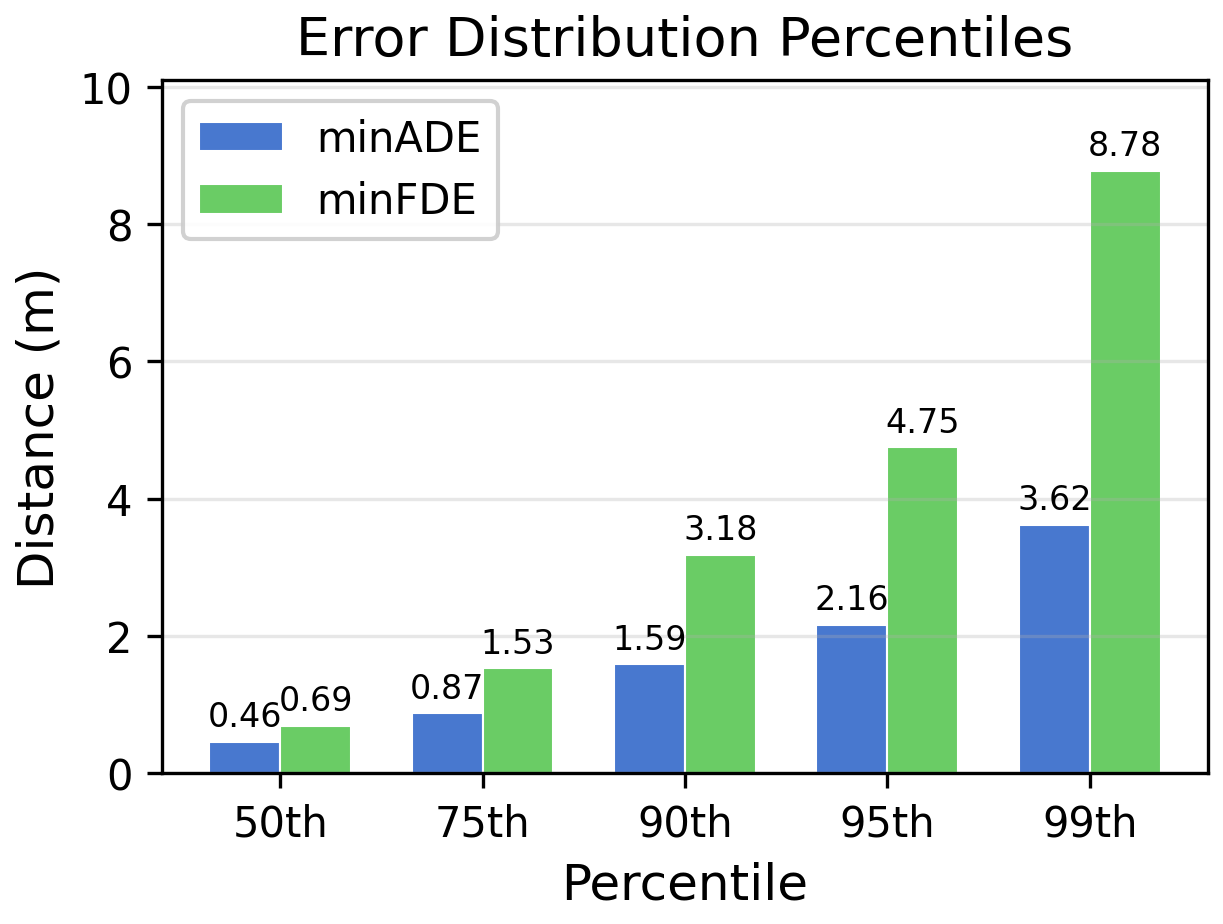
\includegraphics[width=1.0\columnwidth]{Figures/percentile_analysis.png}
\caption{Error distribution analysis showing heavy-tailed behavior on WOMD \texttt{validation\_interactive}.  Median minADE ($0.46\,\text{m}$) is small, but the 95th percentile ($2.16\,\text{m}$) and 99th percentile ($3.62\,\text{m}$) are substantially larger, indicating that a small fraction of interactive scenes drive extreme errors.  These long-tail scenarios are the primary contexts in which rule-aware selection provides the greatest benefit, because the selected trajectory must be executed without a guaranteed geometrically accurate option.}
\label{fig:percentile_analysis}
\end{figure}
